\title{Sammengisleit}
\author{Bergur Snorrason}
\date{\today}

\begin{document}

\frame{\titlepage}

\env{frame}
{
	\frametitle{Sammengisleit}
	\env{itemize}
	{
		\item<1-> \emph{Sammengisleit} (e. \emph{union-find}) er öflug leið til að halda utan um jafngildisflokka tiltekna vensla,
				eða m.ö.o. halda utan um \emph{sundurlæg} mengi.
		\item<2-> Við viljum:
		\env{itemize}
		{
			\item<3-> Bera saman jafngildisflokka mismunandi staka.
			\item<4-> Sameina jafngildisflokka.
		}
		\item<5-> Við tölum um aðgerðirnar \texttt{find(x)} og \texttt{join(x, y)}.
	}
}

\env{frame}
{
	\env{itemize}
	{
		\item<1-> Tökum sem dæmi einstökungasafnið
			$\{\{1\}, \{2\}, \{3\}, \{4\}, \{5\}\}$. 
		\item<2-> \texttt{join(1, 3)} gefur okkur
			$\{\{1, 3\}, \{2\}, \{4\}, \{5\}\}$. 
		\item<3-> \texttt{join(2, 5)} gefur okkur
			$\{\{1, 3\}, \{2, 5\}, \{4\}\}$. 
		\item<4-> \texttt{join(2, 4)} gefur okkur
			$\{\{1, 3\}, \{2, 4, 5\}\}$. 
		\item<5-> \texttt{join(1, 4)} gefur okkur
			$\{\{1, 2, 3, 4, 5\}\}$. 
		\item<6-> Á sérhverjum tímapunkti myndi \texttt{find(x)} skila einhverju staki sem er í sama mengi og \texttt{x}.
		\item<7-> Mikilvægt er að \texttt{find(...)} skilar sama stakinu fyrir sérhvert stak í sérhverjum jafngildisflokki.
		\item<8-> Til dæmis, í þriðja punktinum myndi \texttt{find(1)} og \texttt{find(3)} þurfa að skila sama stakinu.
		\item<9-> Við köllum þetta stak \emph{ráðherra} (e. \emph{representative}) jafngildisflokksins.
	}
}

\env{frame}
{
	\env{itemize}
	{
		\item<1-> Gerum ráð fyrir að tölurnar sem við munum vinna með séu jákvæðar og minni en $n$.
		\item<2-> Við munum þá gefa okkur $n$ staka fylki $p$, þar sem $i$-ta stakið í fylkinu er upphafstillt sem $i$.
		\item<3-> Fylkið $p$ mun nú geyma \emph{foreldri} sérhvers stak.
		\item<4-> Foreldrin mynda keðjur.
		\item<5-> Keðjurnar eru jafngildisflokkarnir.
		\item<6-> Sérhver keðja endar í einhverju staki, sem munu vera ráðherra jafngildisflokksins.
	}
}

\env{frame}
{
	\env{itemize}
	{
		\item<1-> Keðjurnar sem fást með $\{\{0, 2, 4, 5, 9, 10\}, \{1, 3, 6, 11\}, \{7, 8\}\}$ gætu til dæmis verið gefnar með
					$p = [0, 1, 0, 1, 0, 4, 3, 7, 7, 5, 5, 3]$.
		\item<2->[] 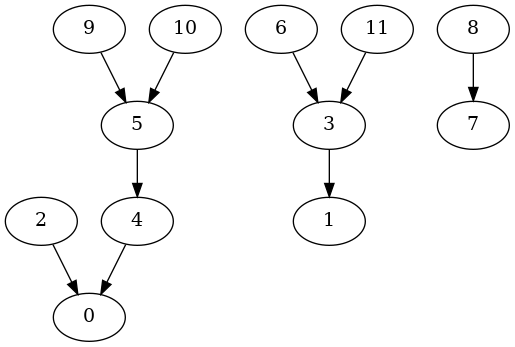
\includegraphics[scale=0.5]{fig/mynd.png}
	}
}

\env{frame}
{
	\env{itemize}
	{
		\item<1-> Til að fá ráðherra flokks tiltekins staks er hægt að fara endurkvæmt upp keðjuna.
		\item<2-> Til að sameina flokka nægir að breyta foreldri ráðherra annars flokksins yfir í
			eitthvert stak hins flokksins (sér í lagi ráðherrann).
		\item<3-> Báðar þessar aðgerðir er auðvelt að útfæra.
	}
}

\env{frame}
{
	\frametitle{Frumstæð sammengisleit}
	\code{code/lst1.c}
}

\env{frame}
{
	\frametitle{Ekki nota frumstæða sammengisleit}
	\env{itemize}
	{
		\item<1-> Við sjáum nú að tímaflækja \texttt{find} er línuleg í lengd keðjunnar, svo 
			þar sem lengd keðjunnar getur verið í versta falli $n$ þá er \texttt{find} með tímaflækjuna $\mathcal{O}($\onslide<2->{$\,n\,$}$)$.
		\item<3-> Fallið \texttt{join} gerir lítið annað en að kalla tvisvar á \texttt{find} svo það er $\mathcal{O}($\onslide<4->{$\,n\,$}$)$.
		\item<5-> Við myndum því aðeins ná að svara $n$ fyrirpsurnum ef $n \leq 10^4$.
		\item<6-> Því er ekki ráðlagt að nota þessa frumstæðu útfærslu.
		\item<7-> Hana má þó bæta.
	}
}

\env{frame}
{
	\frametitle{Keðjuþjöppuð sammengisleit}
	\env{itemize}
	{
		\item<1-> Lykilatriðið í bætingunni er að smækka keðjurnar.
		\item<2-> Í hvert sinn sem við köllum á \texttt{find(...)} þá fletjum við keðjun sem við heimsækjum.
		\item<3-> Þetta er gert með því að setja \texttt{p[x]} sem ráðherra flokks \texttt{x}, í hverju skrefi endurkvæmninnar.
		\item<4-> Þetta köllum við \emph{keðjuþjöppun} (e. \emph{path compression}).
	}
}

\env{frame}
{
	\env{itemize}
	{
		\item<1-> Gefum okkur
			$p = [0, 0, 1, 2, 3, 4, 5, 6, 7]$.
		\item<2-> Ljóst er að \texttt{find(5)} skilar $0$.
		\item<3-> Ef við notum frumstæða sammengisleit breytist $p$ ekki neitt þegar kallað er á \texttt{find}
			en með keðjuþjappaðri sammengisleit þjappast keðjan frá og með $5$ og því fæst
			$p = [0, 0, 0, 0, 0, 0, 5, 6, 7]$.
		\item<4-> Takið eftir að nú er líka styttra í ráðherrann fyrir stök $6$, $7$ og $8$, þó við heimsóttum þau ekki í endurkvæmninni.
	}
}

\env{frame}
{
	\frametitle{Keðjuþjöppað sammengisleit}
	\code{code/lst2.c}
}

\env{frame}
{
	\env{itemize}
	{
		\item<1-> Það er flóknara að lýsa tímaflækju keðjuþjappaðrar sammengisleitar.
		\item<2-> \emph{Á heildina litið} (e. \emph{amortized}) er tímaflækjan er $\mathcal{O}(\alpha(n))$,
					þar sem $\alpha$ er andhverfa \emph{Ackermann} fallsins.
		\item<3-> Fyrir þau $n$ sem við fáumst við er $\alpha(n)$ nánast fast.
		\item<4-> Við ímyndum okkur því alltaf að sammengisleit hafi tímaflækju $\mathcal{O}(\,n\,)$.
	}
}

\env{frame}
{
	\frametitle{\emph{Stærðarmiðuð sameining} (e. \emph{union by size})}
	\env{itemize}
	{
		\item<1-> Þegar við sameinum keðjur þarf að velja hvor ráðherrann verður ennþá ráðherra.
		\item<2-> Við getum þá valið ráðherrann sem hefur fleiri stök í sinni keðju.
		\item<3->[] \selectcode{code/union-find.c}{2}{13}
		\item<4-> Í þessari út færlsu geymir ráðherrann neikvæða tölu, en önnur stök vísa ennþá upp keðjuna.
		\item<5-> Þessi tala svarar til fjölda staka í þeim keðjum sem enda í ráðherranum.
		\item<6-> Svo \texttt{-p[find(x)]} er fjöldi staka í jafngildisflokki \texttt{x}.
	}
}

\env{frame}
{
}


\end{document}
